\documentclass[12pt, dvipdfmx]{beamer}

\renewcommand{\kanjifamilydefault}{\gtdefault}
%%%%%%%%%%%  package  %%%%%%%%%%%
\usepackage{bxdpx-beamer}% dvipdfmxなので必要
\usepackage{pxjahyper}% 日本語で'しおり'したい

\usepackage{amssymb,amsmath,ascmac}

\usepackage{multirow}
\usepackage{bm}

\graphicspath{{../figure/}}

\usepackage{tikz}
\usepackage{xparse}
\usetikzlibrary{shapes,arrows}
%% define fancy arrow. \tikzfancyarrow[<option>]{<text>}. ex: \tikzfancyarrow[fill=red!5]{hoge}
\tikzset{arrowstyle/.style n args={2}{inner ysep=0.1ex, inner xsep=0.5em, minimum height=2em, draw=#2, fill=black!20, font=\sffamily\bfseries, single arrow, single arrow head extend=0.4em, #1,}}
\NewDocumentCommand{\tikzfancyarrow}{O{fill=black!20} O{none}  m}{
\tikz[baseline=-0.5ex]\node [arrowstyle={#1}{#2}] {#3 \mathstrut};}

%目次スライド
% \AtBeginSection[]{
%   \frame{\tableofcontents[currentsection]}
% }
%アペンディックスのページ番号除去
\newcommand{\backupbegin}{
\newcounter{framenumberappendix}
\setcounter{framenumberappendix}{\value{framenumber}}
}
\newcommand{\backupend}{
\addtocounter{framenumberappendix}{-\value{framenumber}}
\addtocounter{framenumber}{\value{framenumberappendix}} 
}

%%%%%%%%%%%  theme  %%%%%%%%%%%
\usetheme{Copenhagen}
% \usetheme{Metropolis}
% \usetheme{CambridgeUS}
% \usetheme{Berlin}

%%%%%%%%%%%  inner theme  %%%%%%%%%%%
% \useinnertheme{default}

% %%%%%%%%%%%  outer theme  %%%%%%%%%%%
\useoutertheme{default}
% \useoutertheme{infolines}

%%%%%%%%%%%  color theme  %%%%%%%%%%%
%\usecolortheme{structure}

%%%%%%%%%%%  font theme  %%%%%%%%%%%
\usefonttheme{professionalfonts}
%\usefonttheme{default}

%%%%%%%%%%%  degree of transparency  %%%%%%%%%%%
%\setbeamercovered{transparent=30}

% \setbeamertemplate{items}[default]

%%%%%%%%%%%  numbering  %%%%%%%%%%%
% \setbeamertemplate{numbered}
\setbeamertemplate{navigation symbols}{}
\setbeamertemplate{footline}[frame number]


\title{絡み合いとプラトー弾性率}
% \subtitle{ ~ はじめに ~}
\author[東亞合成 佐々木]{佐々木 裕\thanks{hiroshi\_sasaki@mail.toagosei.co.jp}}
\institute[東亞合成]{東亞合成株式会社}
\date{\today}

\begin{document}

%%%%%
% 1 P
%%%%%
\maketitle

\section{Z1 code, PPA}
\subsection{Z1 code}
\begin{frame}{Z1 code}
    \centering
        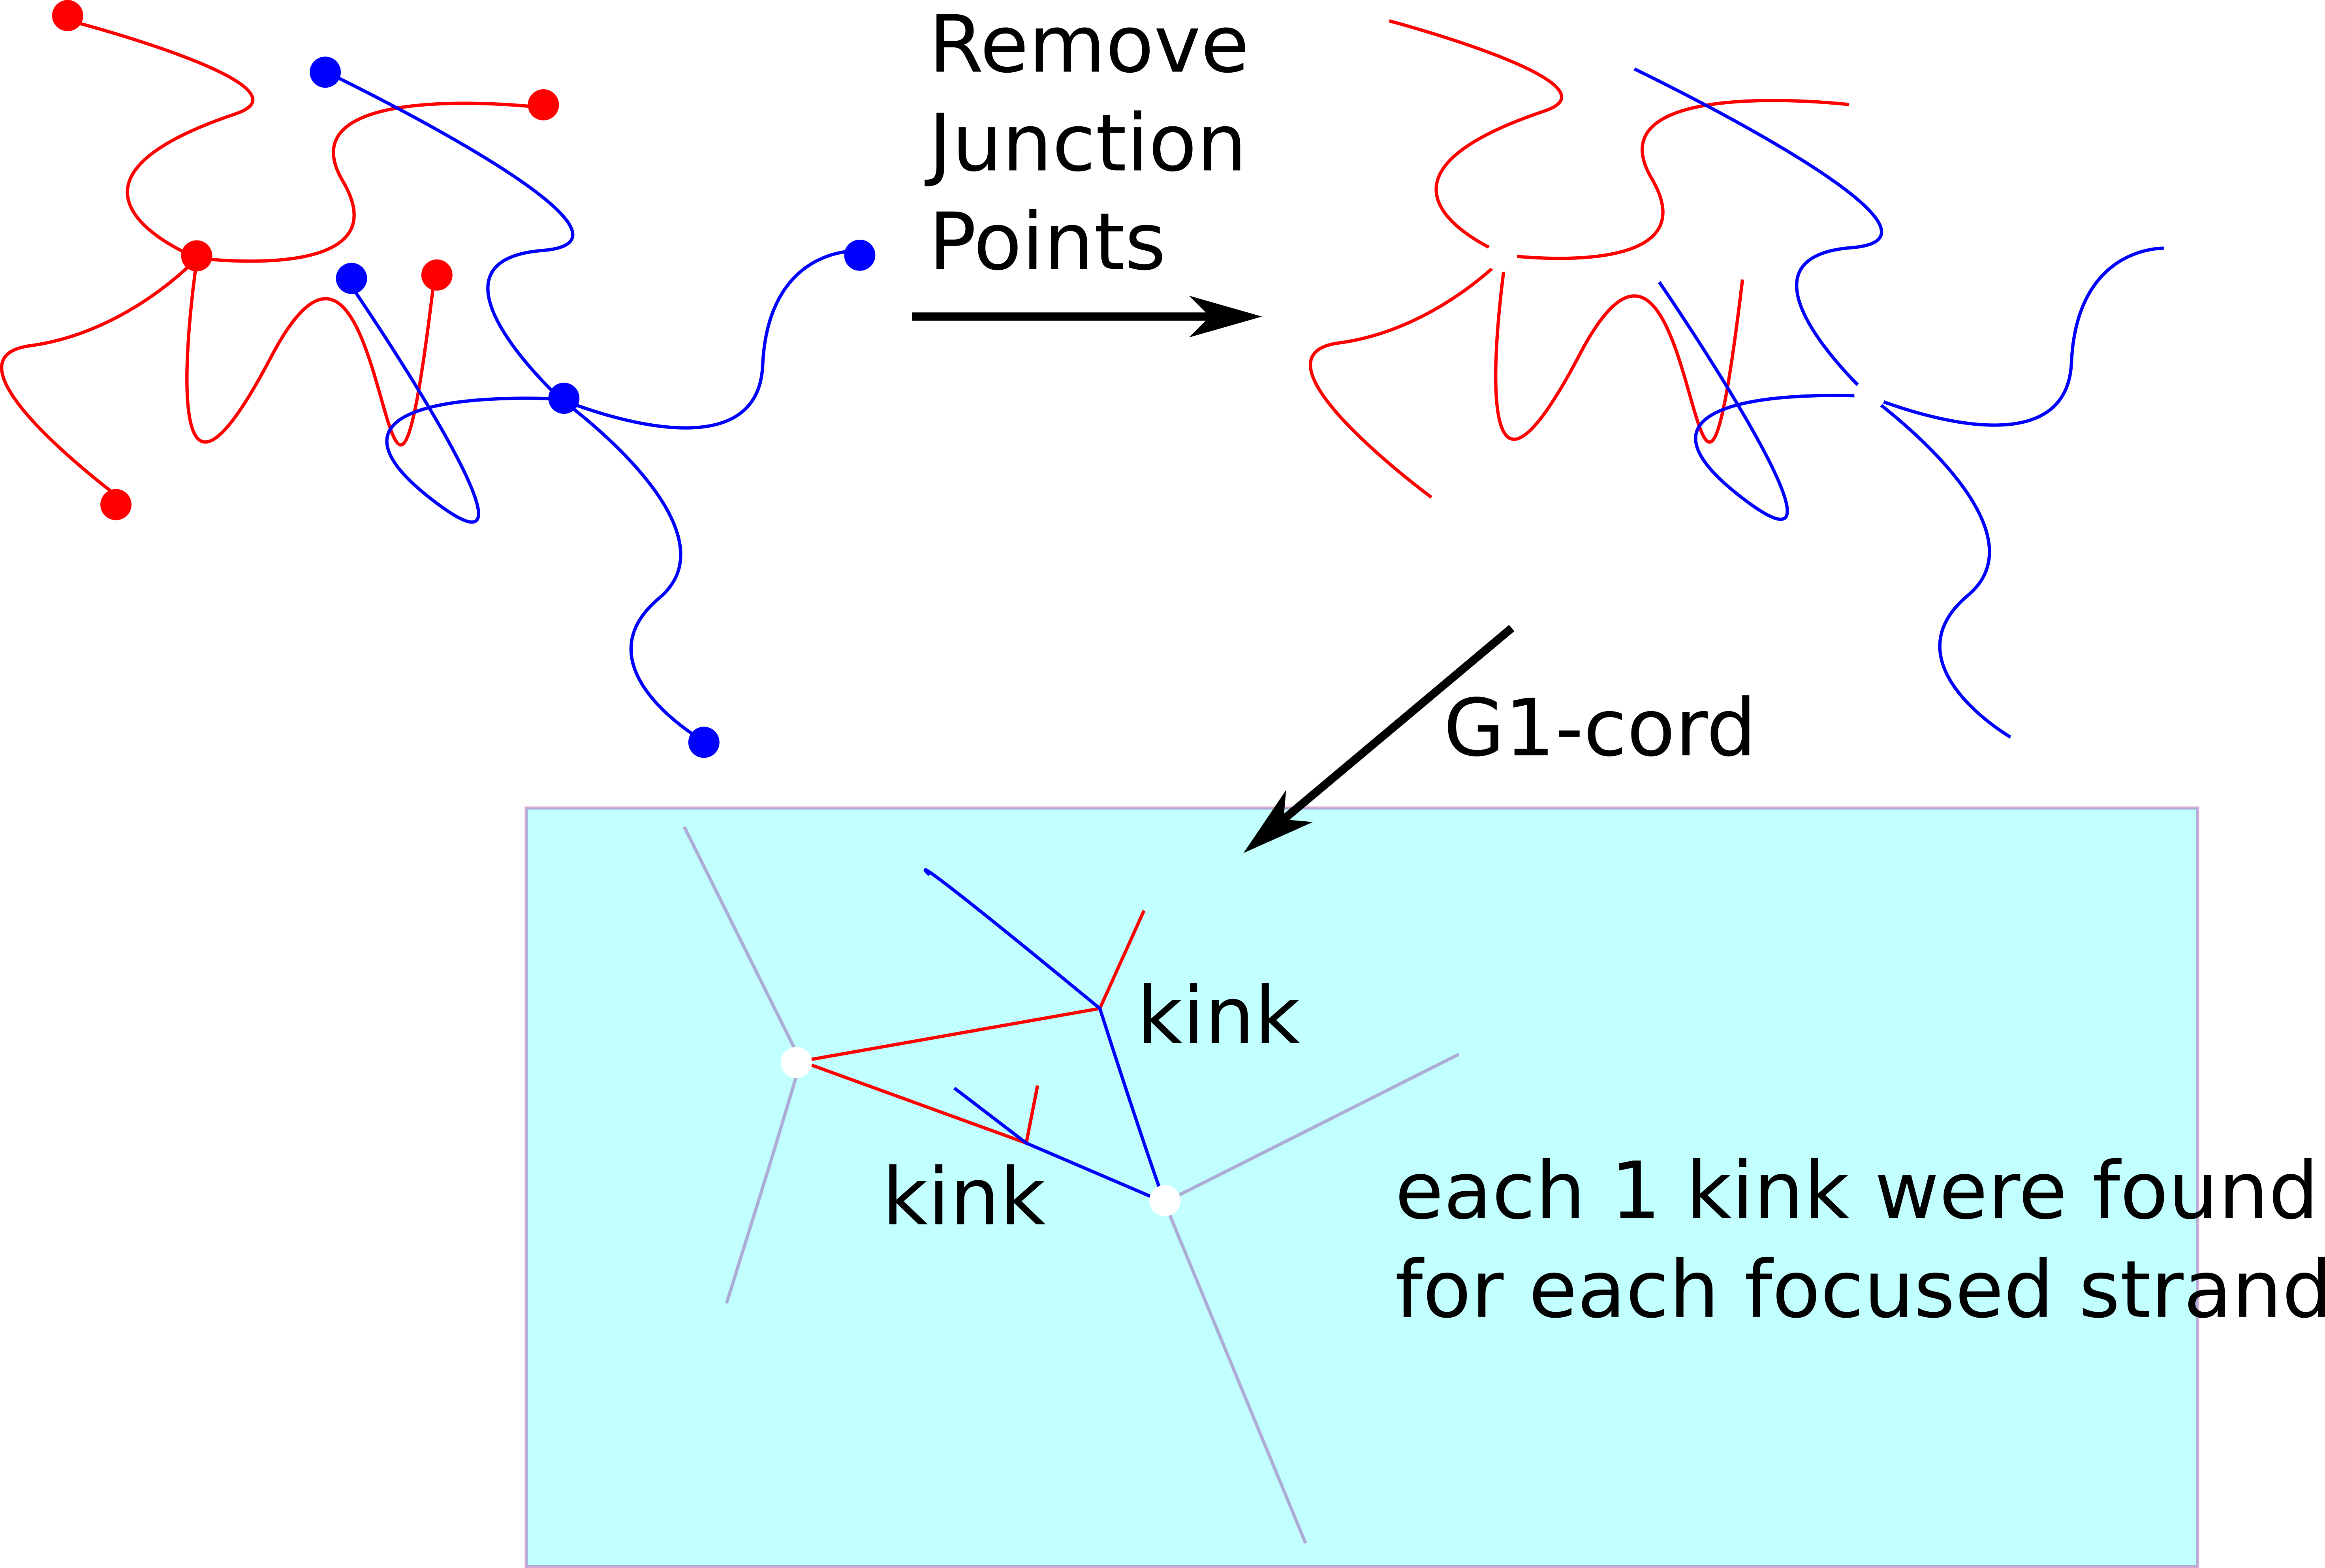
\includegraphics[width=.95\textwidth]{z1cord.png}
\end{frame} 

\subsection{Comparison of Z1 vs. PPA}
\begin{frame}
    \frametitle{Comparison of Z1 vs. PPA}
    \begin{columns}[T, onlytextwidth]
        \column{.4\linewidth}
            \begin{itemize}
                \item 右図のような比較から、二倍程度は妥当かと。
                \item 次ページにあるネットワークでの比較でも明らかにPPA由来の経路長は長い
                \item これと、プラトー弾性率との関係はよくわかりません。
            \end{itemize}

        \column{.58\linewidth}
        \centering
        \includegraphics[width=\textwidth]{z1_PPA.png}
    \end{columns}
\end{frame}

\subsection{Example for Networks}
\begin{frame}
    \frametitle{Example for NW}
    \begin{columns}[T, onlytextwidth]
        \column{.28\linewidth}
        \column{.35\linewidth}
        \centering
            Z1 cord
        \column{.35\linewidth}
        \centering
            PPA
    \end{columns}
    \begin{columns}[c, onlytextwidth]
        \column{.28\linewidth}
        NPT\\
        絡み合い小
        \column{.35\linewidth}
        \centering
            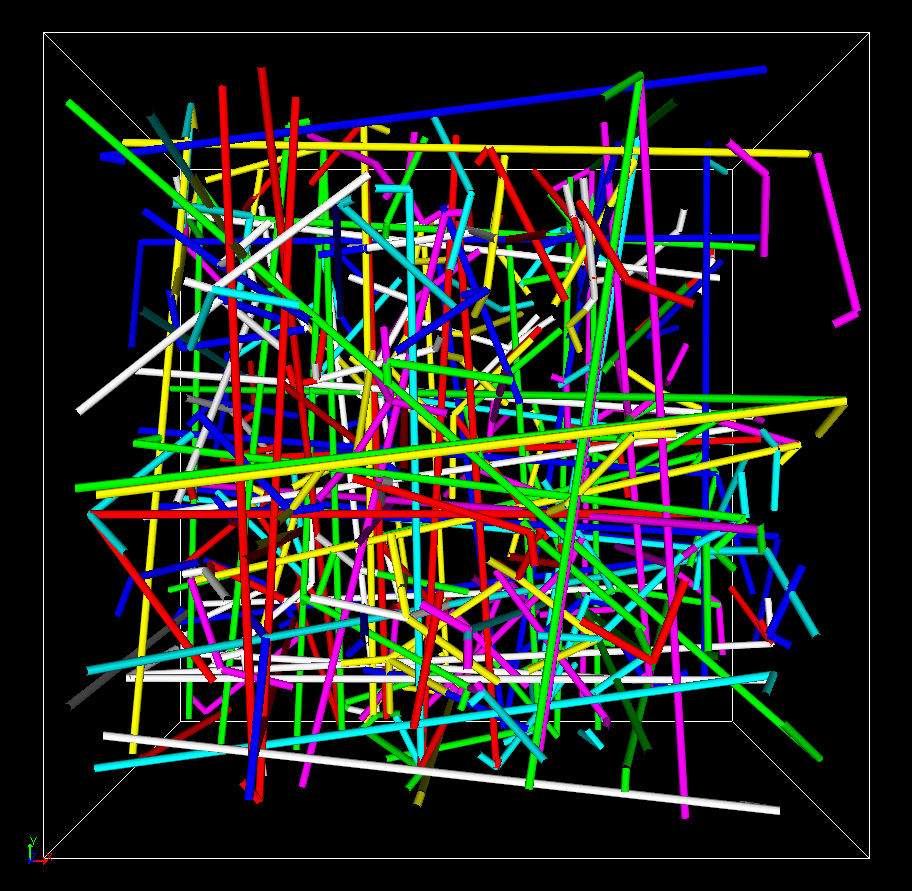
\includegraphics[width=.8\textwidth]{z_cord_NPT_4Chain.png}
        \column{.35\linewidth}
        \centering
            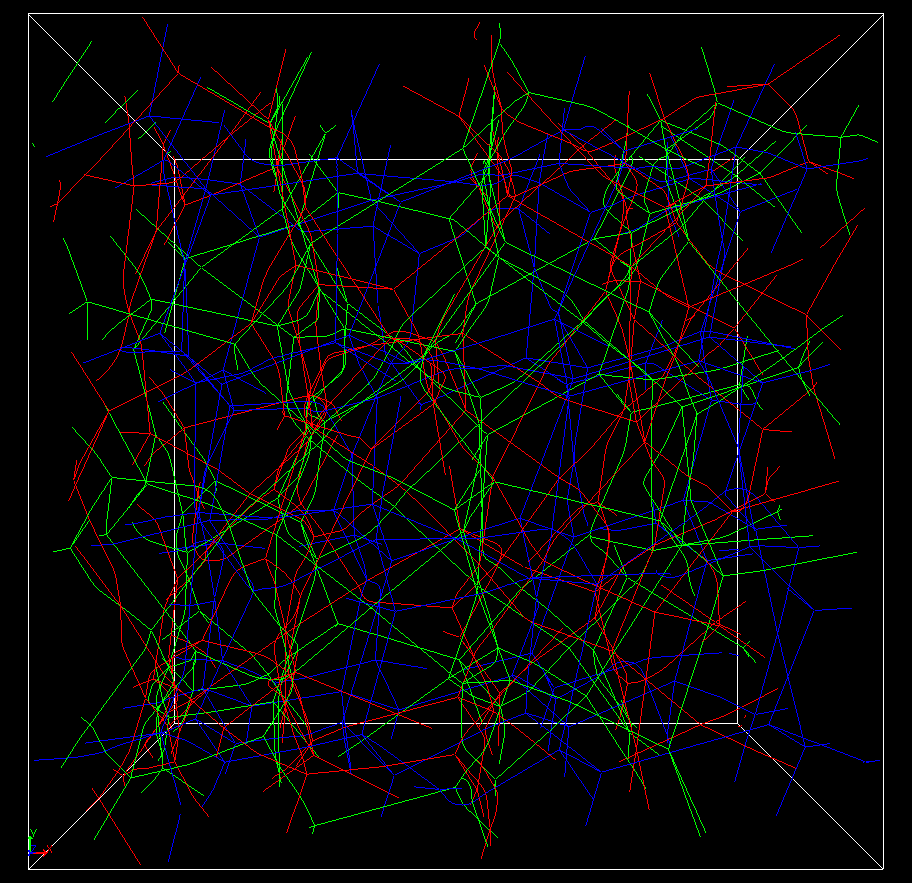
\includegraphics[width=.8\textwidth]{NPT_PPA.png}
    \end{columns}
    \vspace{3mm}
    \begin{columns}[c, onlytextwidth]
        \column{.28\linewidth}
        NVT\\
        自然な絡み合い
        \column{.35\linewidth}
        \centering
            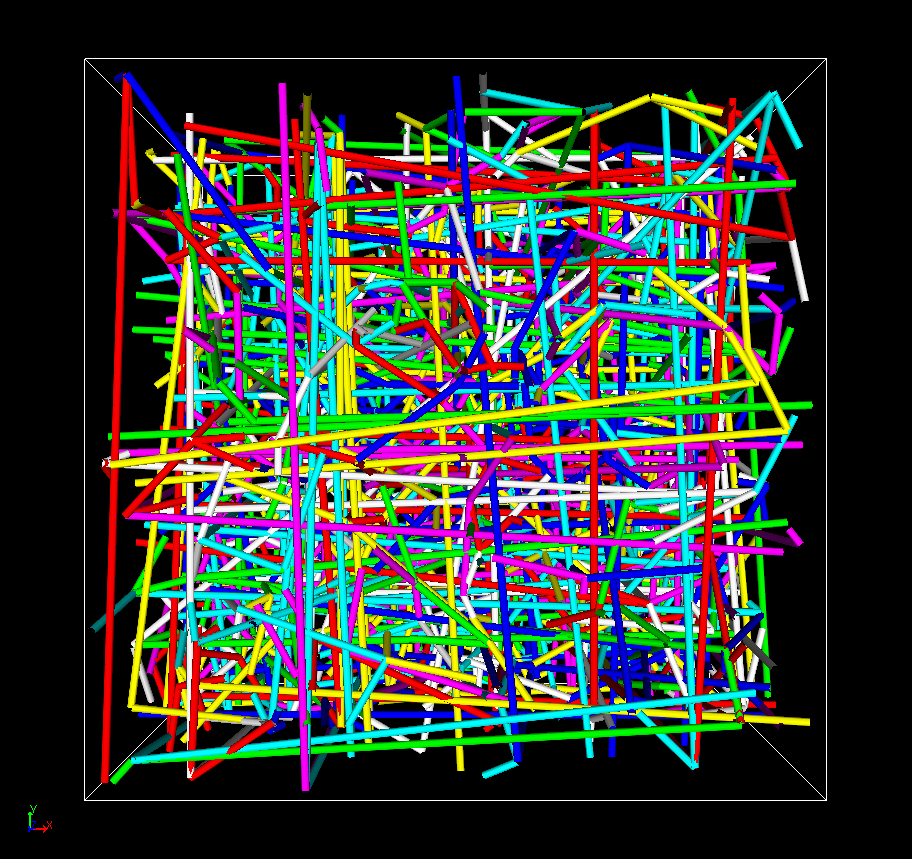
\includegraphics[width=.8\textwidth]{z_cord_4Chain.png}
        \column{.35\linewidth}
        \centering
            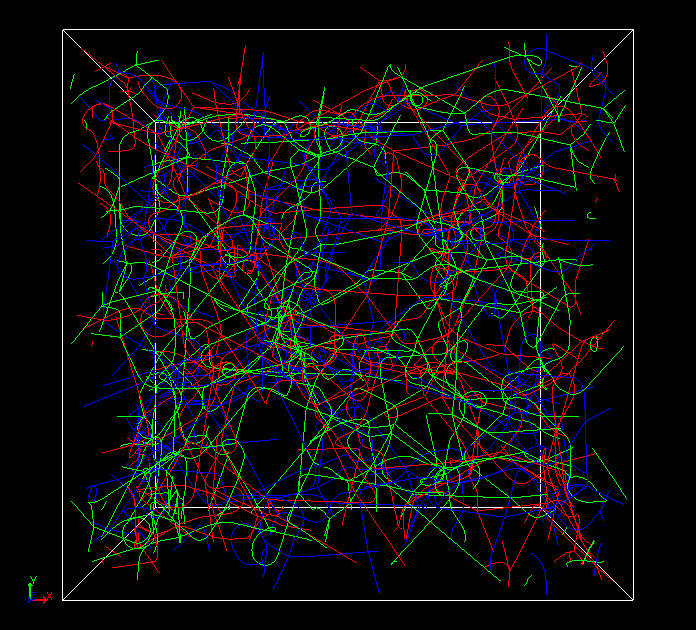
\includegraphics[width=.8\textwidth]{N48_f4_PPA.png}
    \end{columns}
\end{frame}

\section{ゴムのモデル化}
\subsection{Classical Theory of Rubber Elasticity}
\begin{frame}
    \frametitle{Classical Theory of Rubber Elasticity}
        \vspace{-2mm}
		\begin{block}{Free Energy Density of Rubbers against Strain invariant}
			\vspace{-6mm}
			% 非圧縮性条件から第3不変量がおちて、
			\scriptsize
			\begin{align*}
				\dfrac{F}{V} = W 
				% &= \sum_{i,j = 0}^{\infty} C_{ij}(I_1-3)^i(I_2-3)^j \\[-2mm]
				&= C_0 + \underbrace{{\color{green}C_1(I_1-3)} + {\color{red}C_2(I_2-3)}}_{\color{red}Mooney-Rivlin Model} + \sum_{i,j = 1}^{\infty} C_{ij}(I_1-3)^i(I_2-3)^j
			\end{align*}  
		\end{block}
		\vspace{-5mm}
		\begin{columns}[T, onlytextwidth]
			\column{.48\linewidth}
				\begin{exampleblock}{Neo-Hookean Model}
					\vspace{-6mm}
					% 第1不変量のみを対象
						\scriptsize
						\begin{align*}
							&W = C_1 (I_1-3) \\
							&\text{against Uniaxial elongation} \\
							&\sigma_{nom} = 2 C_1\left(\lambda - \dfrac{1}{\lambda^2}\right) = G \left(\lambda - \dfrac{1}{\lambda^2}\right)
						\end{align*}
				\end{exampleblock}
			\column{.48\linewidth}
				\begin{alertblock}{Mooney-Rivlin Model}
					\vspace{-6mm}
					% 高次の項をおとす
					\scriptsize
					\begin{align*}
						&W = C_1 (I_1-3) + C_2(I_2-3) \\
						&\text{against Uniaxial elongation} \\
						&\sigma_{nom} = 2 \left(C_1 + C_2\dfrac{1}{\lambda} \right) \left(\lambda - \dfrac{1}{\lambda^2}\right)
					\end{align*}
				\end{alertblock}
		\end{columns}
		\vspace{-1mm}
		\begin{block}{With or without Junction Poinits fluctuation}
			\vspace{1mm}
			\begin{columns}[T, onlytextwidth]
				\column{.48\linewidth}
				\small
				\color{blue}{Affine Network Model
				\footnote{
					\tiny{P.J. Flory, Principles of Polymer Chemistry, (1953)}
				}
				}
				\vspace{-2mm}
				\scriptsize
				\begin{align*}
					% &\text{Affine Network Model}\\
					&G_{affine} = \nu k_B T  \\
					&\text{$\nu$: Number density of strands in the system}
				\end{align*}
				\column{.48\linewidth}
				\small
				\color{magenta}{Phantom Network Model
				\footnote{
					\tiny{H.M. James, E.J. Guth, Chem. Phys., 21, 6, 1039 (1953)}
				}
				}
				\vspace{-2mm}
				\scriptsize
				\begin{align*}
					% &\text{Phantom Network Model}\\
					&G_{phantom} = \nu k_B T \left(1 - \dfrac{2}{f}\right) \\
					&\text{$f$: Functionality of Junction Points}
				\end{align*}
				\normalsize
			\end{columns}
		\end{block}
\end{frame}


\begin{frame}
	\frametitle{Constraint Factors for Junction Points and Strands}
		\vspace{-2mm}
		\begin{alertblock}{Vicinity of Junction Point}
			\begin{columns}[totalwidth=1\textwidth]
				\column{.75\textwidth}
				\vspace{-3mm}
				\begin{itemize}
					\item Junction points are surrounded by many of \alert{adjacent strands(x in fig.).}
					\item %Because of surrounding strands, 
					Fluctuation of junctions are \alert{suppressed}. 
				\end{itemize}
				\column{.22\textwidth}
				\centering
				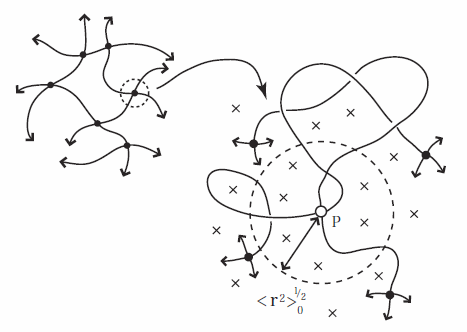
\includegraphics[width=\textwidth]{JP_vicinity.png}
			\end{columns}
		\end{alertblock}
		\vspace{-1mm}
		Storage modulus $G$ is \alert{combination of $G_c$ and $G_e$}
		\vspace{-1mm}
			\begin{columns}[totalwidth=1\textwidth]
				\column{.65\textwidth}
				\begin{itemize}
					\item Constrained Junction Model
					\begin{itemize}
						\item Constraints are reduced and $G$ approaches to $G_c$.\footnote{\tiny{P.J.Flory, J.Chem.Phys., 66, 12, 5720 (1977)}}
					\end{itemize}
					\item Topological relationships
					\begin{itemize}
						\item Contribution of entanglement.\footnote{\tiny{D.S.Pearson and W.Graessley, Macromol., 11, 3, 528 (1978)}}
						\vspace{-2mm}
						\scriptsize
						\begin{align*}
							G_e = T_e G_N^0
						\end{align*}
					\end{itemize}
				\end{itemize}
				\column{.3\textwidth}
				\vspace{-2mm}
				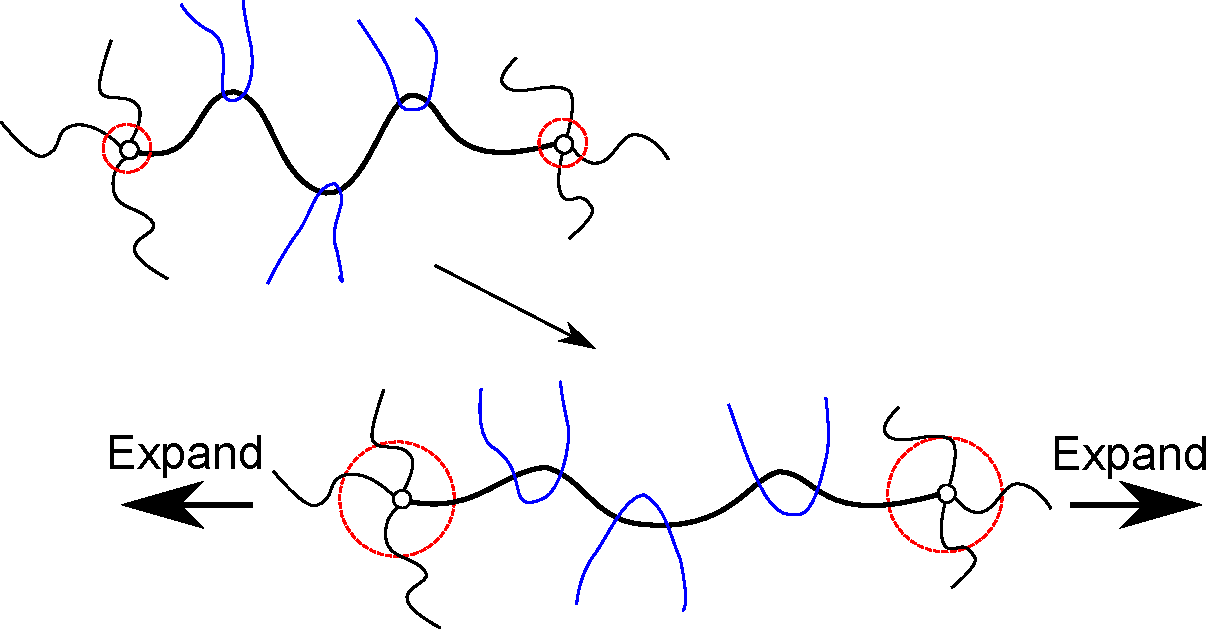
\includegraphics[width=\textwidth]{Constrained_Juntion.pdf}

				\vspace{3mm}
				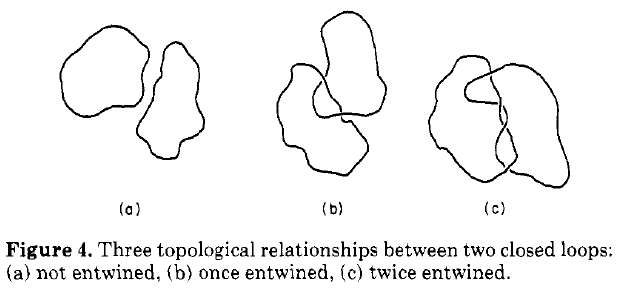
\includegraphics[width=\textwidth]{topological_effect_ring.png}
			\end{columns}
		% \end{block}
\end{frame}

\setcounter{footnote}{0}

\subsection{Recent approach for Constraints (Entanglements)}
\begin{frame}
	\frametitle{Recent approach for Constraints (Entanglements)}
	
		\begin{itemize}
			\item Diffused-Constraint Model
			\begin{itemize}
				\item Confining potential affect all points along the chain.\footnote{\tiny{A. Kloczkowski, J.E. Mark, B. Erman, Macromol., 28, 5089 (1995)}}
			\end{itemize}
			\item Nonaffine Tube Model
			\begin{itemize}
				\item Improved model of "Edwards' Tube Model".\footnote{\tiny{M. Rubinstein, S. Panyukov, Macromol., 30, 25, 8036 (1997)}}
			\end{itemize}
			\item Slip-tube Model
			\begin{itemize}
				\item A pairwise interaction of chains is introduced.\footnote{\tiny{M. Rubinstein, S. Panyukov, Macromol., 35, 6670 (2002)}}
			\end{itemize}
		\end{itemize}

		% \begin{alertblock}{Slip-tube Model(Simple analytical appoximation)}
			\begin{columns}[totalwidth=1\textwidth]
				\column{.7\textwidth}
				\scriptsize
				\begin{align*}
					&f^*(\lambda^{-1}) = G_c + \dfrac{G_e}{0.74 \lambda + 0.61 \lambda^{-1/2} - 0.35} \\
					&G_c = \nu k_B T \left(1-\dfrac{2}{\phi} \right), \quad G_e = \dfrac{4}{7} \nu k_B T L \\
					% &\text{where $\nu$ is the number density of network chains,} \\
					& \text{L is the number of slip-links per network chain}
				\end{align*}
				\column{.25\textwidth}
				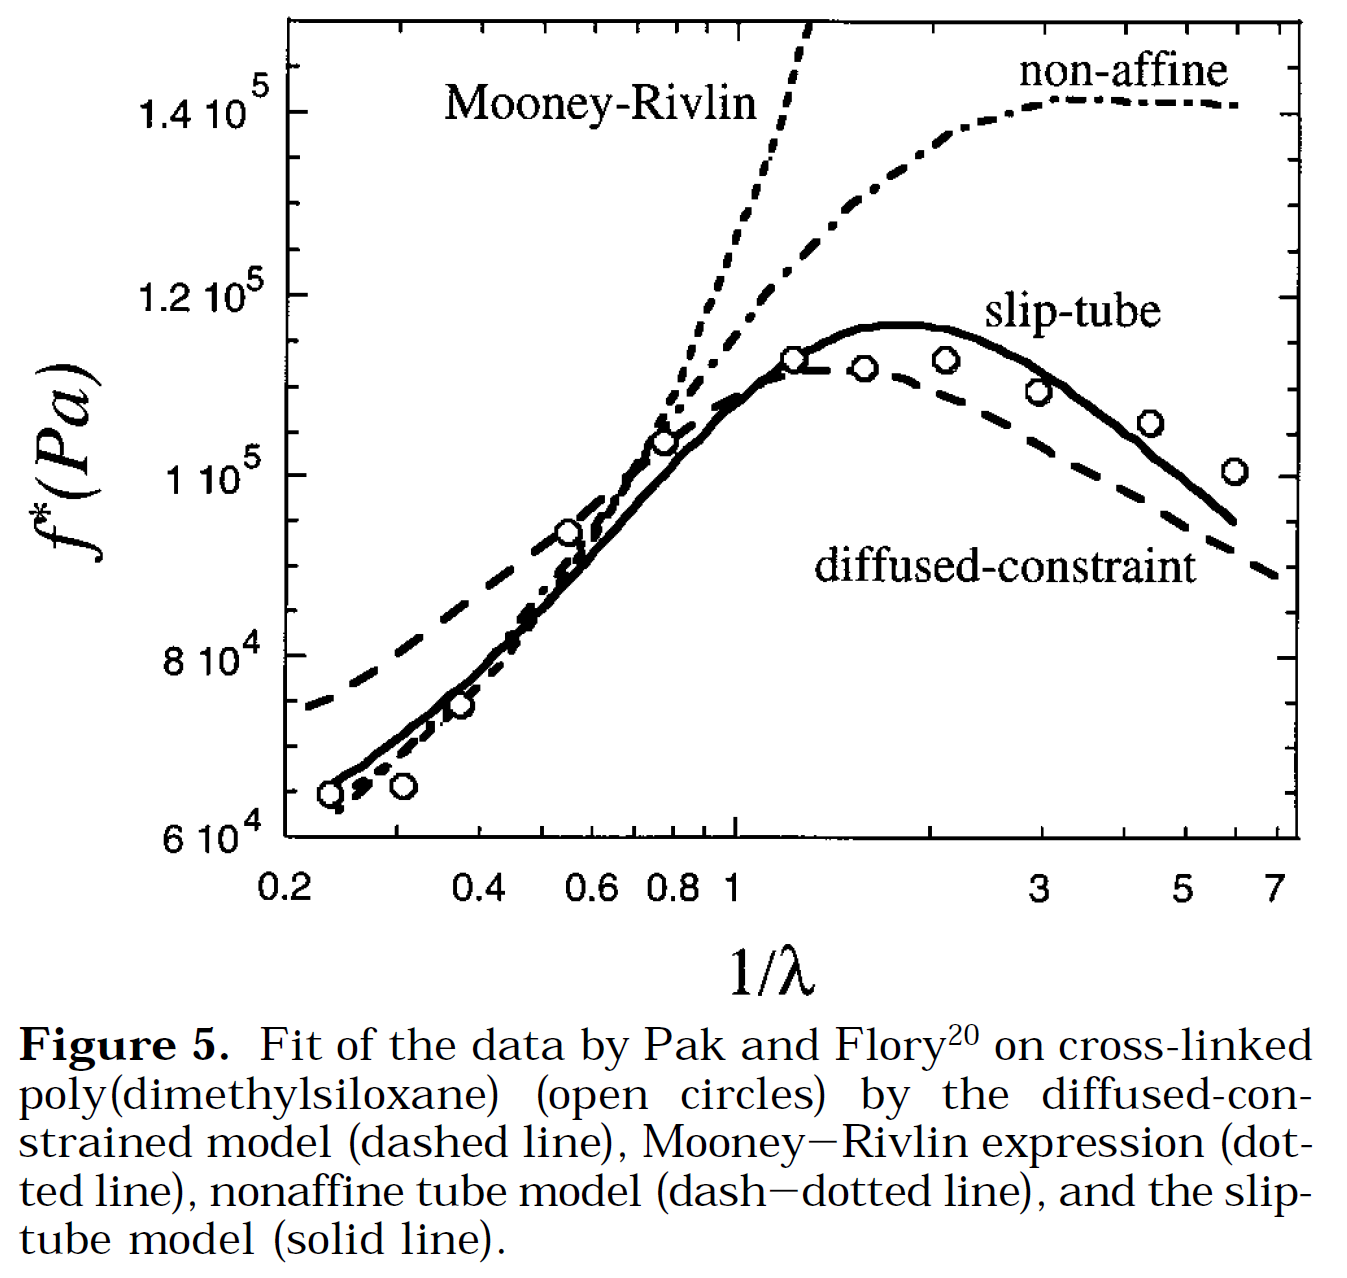
\includegraphics[width=.9\textwidth]{NW_model_rubinstein.png}
			\end{columns}
		% \end{alertblock}	
\end{frame}

\section{NWシミュレーションの結果}

\begin{frame}
    \frametitle{ランダムネットワークの絡み合い解析: Z1-code}
        \vspace{-2mm}
        \begin{columns}[onlytextwidth]
            \column{.4\linewidth}
                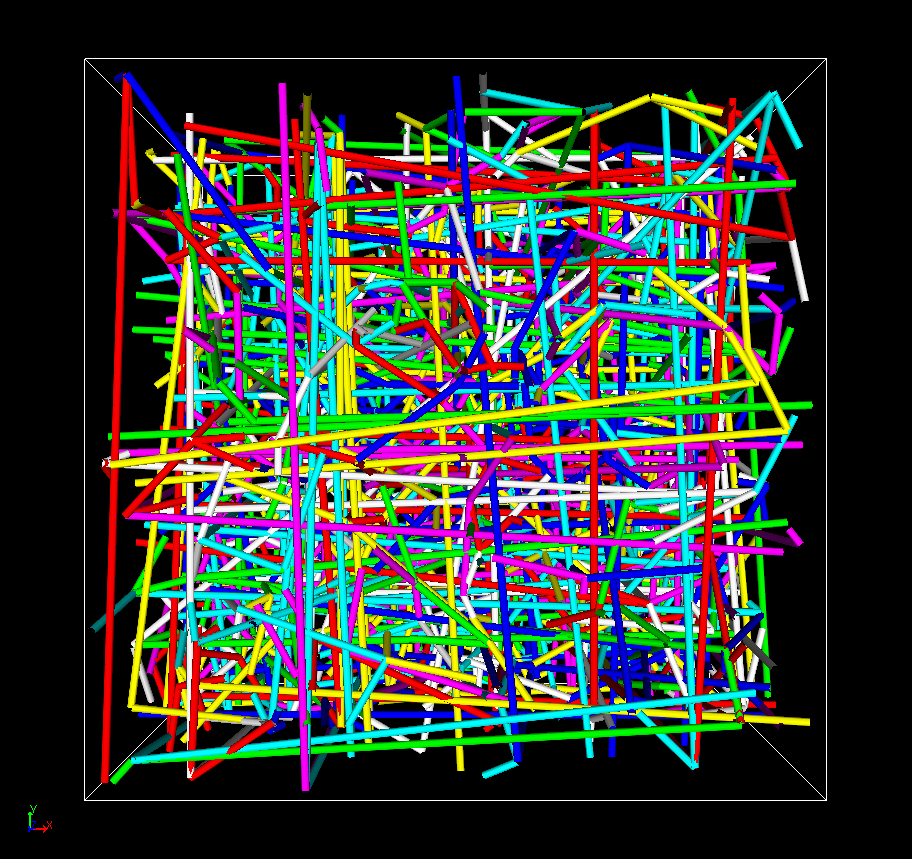
\includegraphics[width=.9\textwidth]{z_cord_4Chain.png}

                Z1-code での絡み合い
            \column{.56\linewidth}
            \begin{block}{ホモポリマーとの比較}
                \begin{itemize}
                    \item Z は一本鎖あたりの絡み合い
                    \item 今回のネットワークは、\\ホモポリマーと同等
                \end{itemize}
                \scriptsize
                \begin{center}
                    \begin{tabular}{c||c|c} \hline
                        &Homo & 4 Chain NW \\ \hline \hline
                        Segments& 50& 48 \\ \hline
                        Chains & 200& 768 \\ \hline
                        Entanglements& 204& 800\\ \hline
                        Entangled Chains&134&557 \\ \hline
                        \alert{$<Z>_{Z1}$}&\alert{1.02}& \alert{1.04}\\ \hline
                    \end{tabular}
                \end{center}
            \end{block}
        \end{columns}
    \begin{alertblock}{Z1-codeとは}
        \begin{itemize}
            \item 絡み合いを可視化するアルゴリズム\footnote{
                M. Kröger, Comput. Phys. Commun. 168, 209 (2005)
                % \begin{itemize}
                %     \item M. Kröger, Comput. Phys. Commun. 168, 209 (2005)
                %     \item S. Shanbhag, M. Kröger, Macromolecules 40, 2897(2007)
                %     \item R. Hoy, K. Foteinopoulou, M. Kröger, Phys. Rev. E, 31803 (2009)
                % \end{itemize}
            }
        %    N.C. Karayiannis, M. Kröger, Int. J. Mol. Sci. 10, 5054 (2009)
        \end{itemize}
    \end{alertblock}
\end{frame}

\begin{frame}
    \frametitle{絡み合いの効果について}
	\vspace{-3mm}
	\begin{alertblock}{Entanglement in Slip-tube Model}
		% \begin{columns}[onlytextwidth]
		% 	\column{.8\linewidth}
			\small
			Rubinstein らの先行研究\footnote{
				\scriptsize{M. Rubinstein, S. Panyukov, Macromolecules, 35, 6670 (2002)}
				}
			\vspace{-3mm}
			\scriptsize
			\begin{align*}
				&G_c = \nu k_B T \left(1-\dfrac{2}{\phi} \right), \quad G_e = \dfrac{4}{7} \nu k_B T L \\
				% &\text{where $\nu$ is the number density of network chains,} \\
				& \text{and L is the number of slip-links per network chain}
			\end{align*}
	\end{alertblock}
	% \vspace{-1mm}
	\begin{columns}[onlytextwidth]
		\column{.2\linewidth}
			\centering
			\vspace{3mm}
			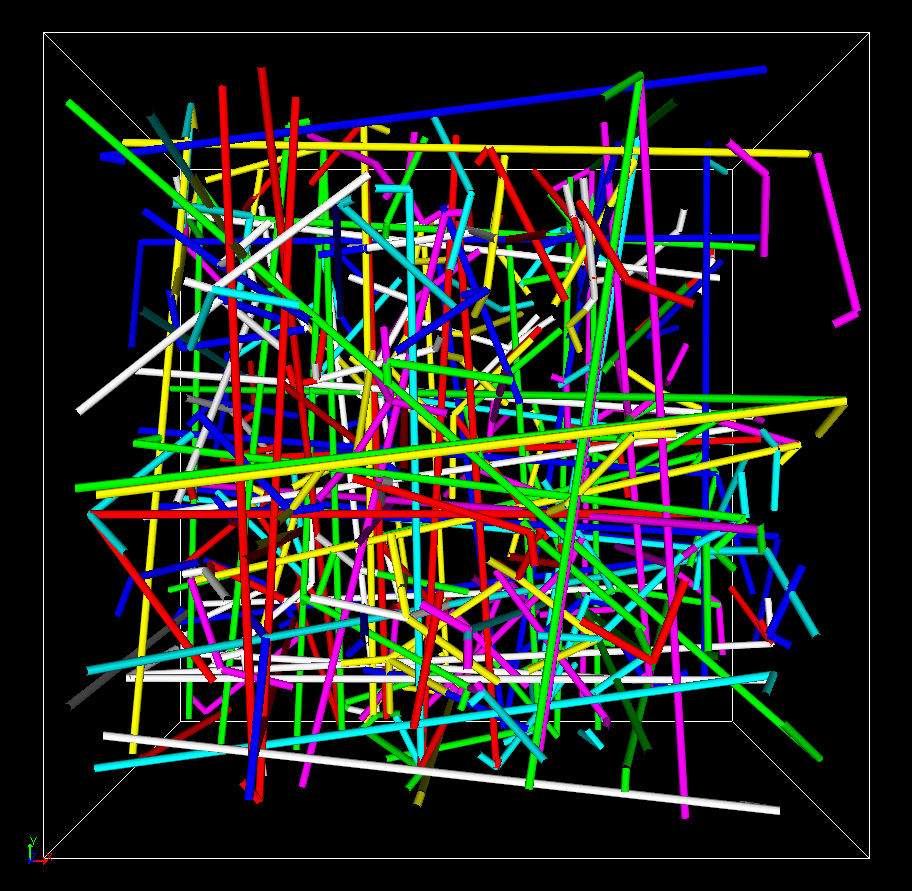
\includegraphics[width=.8\textwidth]{z_cord_NPT_4Chain.png}
			\vspace{2mm}
				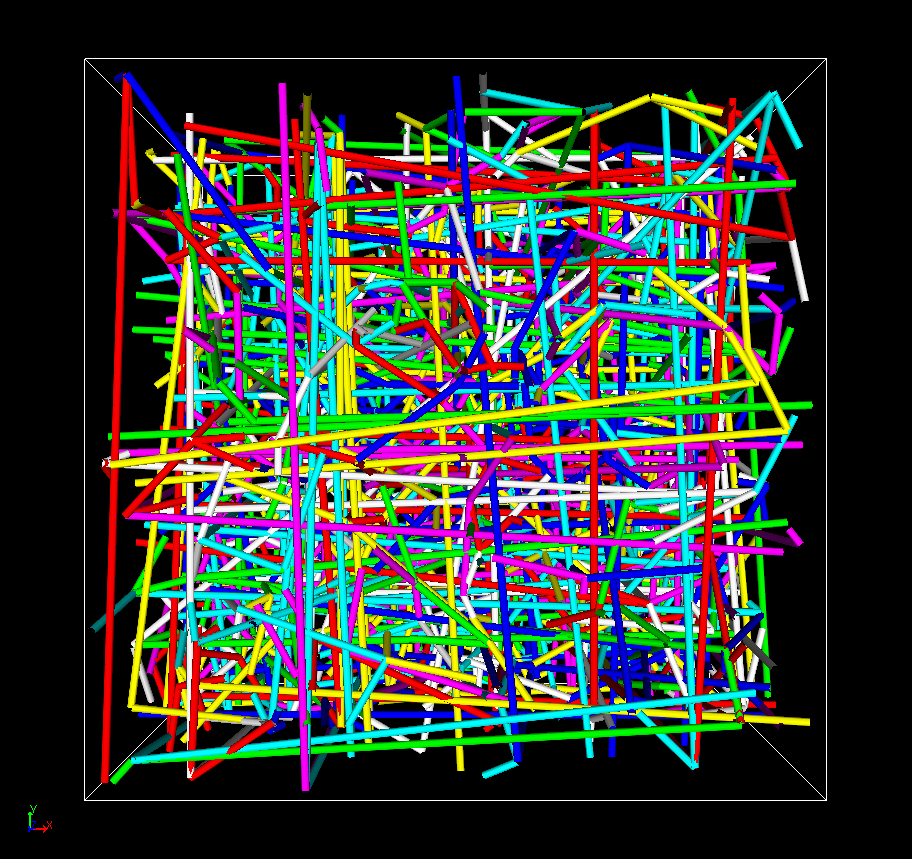
\includegraphics[width=.8\textwidth]{z_cord_4Chain.png}
		\column{.8\linewidth}
		\scriptsize
			\centering
			\begin{tabular}{c|c|c} \hline
				&NPT & NVT \\ \hline \hline
				\textcolor{blue}{Chains, $\nu$} & \multicolumn{2}{|c}{\textcolor{blue}{768, 0.018}}\\ \hline
				% \textcolor{blue}{$\nu$}& \multicolumn{2}{|c}{\textcolor{blue}{0.018}}\\ \hline
				\textcolor{blue}{$G_c = \nu \times (1-2/4)$}&\multicolumn{2}{|c}{\textcolor{blue}{0.009}} \\ \hline \hline
				Entanglements& 278& 800\\ \hline
				Entangled Chains&249&557 \\ \hline
				\textcolor{green}{L} & \textcolor{green}{278/768=0.36} & \textcolor{green}{800/768=1.04} \\ \hline
				$G_e=4/7 \times \nu \times L $ & 0.004 & 0.011 \\ \hline \hline
				\alert{$G_{calcd.}=G_c + G_e$} & \alert{0.013} & \alert{0.020} \\ \hline \hline
				\textcolor{blue}{$G_{measd.}$} & \textcolor{blue}{0.013} & \textcolor{blue}{0.022} \\ \hline
			\end{tabular}
	\end{columns}
\end{frame}

\end{document}